%!TEX encoding = UTF-8 Unicode
%!TEX TS-program = xelatex
%!BIB TS-program = biber
\documentclass[a4paper,12pt]{article}
\usepackage[margin=22mm]{geometry}
\usepackage{fontspec,xltxtra,polyglossia,titling,graphicx}
\usepackage{caption}  \captionsetup[table]{skip=6pt}
\usepackage{verbatim,synttree,multicol,booktabs,gb4e}
\noautomath
\usepackage[colorlinks,urlcolor=blue,citecolor=blue,linkcolor=blue]{hyperref}
\setmainfont[Mapping=tex-text]{Times New Roman} % or another similar font
\usepackage[backend=biber, style=authoryear, citestyle=authoryear-comp, maxcitenames=2, maxbibnames=50, language=auto, isbn=false, doi=true]{biblatex} % may produce a warning
\frenchspacing


\title{Redes Neuronales MLP: Caso de estudio} % replace with title of your term paper
\author{Autor 1 \\ Autor 2} % Nombres de los integrantes del equipo
\newcommand{\Coursecode}{Clase de Inteligencia Artificial \\ Proyecto del tercer parcial} % replace with course code and name
\newcommand{\Semester}{Mayo 2023}

\setdefaultlanguage{english}

\addbibresource{sample.bib}

\newcommand{\tig}[1] {\fontspec{Abyssinica SIL} #1} % example fontspec for Tigrinya

\hyphenation{lem-mat-iz-at-ion uni-code}

\begin{document}
\begin{center} \vfill
\thispagestyle{empty}
\textbf{\Large Universidad Panamericana}

{\large Facultad de Ingeniería  \vfill

\Coursecode

\Semester} \vfill


\includegraphics[width=80mm]{pics/UP_logo.png} \vfill

\emph{\Large \thetitle} \vfill

{\large \theauthor} \vfill

\end{center} \clearpage
 \maketitle

\section{Instrucciones para ejecutar el código} % así se crea una sección
\label{sec:intro} % esta es la etiqueta de la sección 
Aquí va un texto.

Esto es un pie de página.\footnote{Leipzig Glossing Rules: \url{https://www.eva.mpg.de/lingua/resources/glossing-rules.php}}

Las ecuaciones se referencian así \ref{eq:lix}. Y se escriben así 

\begin{equation} \label{eq:lix}[h]
Lix=\frac{W}{S}+\frac{L \cdot 100}{W}
\end{equation}

Las referencias a tablas se ven así \ref{tab:pct}. Y la tabla está en tabla1.tex

\begin{table}[h]
\centering
\caption{Caption at the top of a table.}
\label{tab:pct}
\begin{tabular}{lrr}
\toprule
{} &     f &     m \\
Word     &       &       \\
\midrule
beat     &  31.7 &  68.3 \\
bloke    &  36.0 &  64.0 \\
cat      &  65.4 &  34.6 \\
clothes  &  69.1 &  30.9 \\
cool     &  30.3 &  69.7 \\
crap     &  35.5 &  64.5 \\
football &  24.1 &  75.9 \\
kiss     &  81.5 &  18.5 \\
love     &  72.2 &  27.8 \\
model    &  88.2 &  11.8 \\
music    &  45.8 &  54.2 \\
phone    &  70.9 &  29.1 \\
\bottomrule
\end{tabular}
\end{table}

La referencia a una sección  se ve así \ref{sec:intro}

Las referencias a la bibliografía se ven así  \parencite{Kopka04,Mittelbach04,Van_Dongen12}. La bibliografía está en este archivo .bib file. La bibliografía se puede obtener de google scholar en formato bibtex; sólo habrá que copiar y pegar en el archivo y luego hacer referencia aquí.

\footnote{Una guía a BibLaTeX: \url{http://tug.ctan.org/info/biblatex-cheatsheet/biblatex-cheatsheet.pdf}} 

\section{Definición del problema}
\label{sec:def}
Aquí va la definición del problema

\section{Conjunto de datos}
\label{sec:datos}
Aquí va la descripción del conjunto de datos

\section{Clasificación}
\label{sec:clas}
Aquí va todos los experimentos de clasificación 

\subsection{Red Neuronal de base}
\label{sec:clasRedBase}
Aquí va la descripción de la red neuronal de base

\subsection{Búsqueda de hiper-parámetros}
\label{sec:clasHiper}
Aquí va la descripción de la búsqueda de hiper-parámetros

\subsection{Red Neuronal Optimizada}
\label{sec:clasRedOpt}
Aquí va la descripción de la red neuronal con mejor rendimiento

\subsection{Análisis de las redes neuronales}
\label{sec:clasAn}
Aquí va la descripción del análisis de la red neuronal con mejor rendimiento.

Las referencias a figuras se ven así \ref{fig:bp}. Las figuras están todas en la carpeta pics

\begin{figure}[htbp] \begin{center}
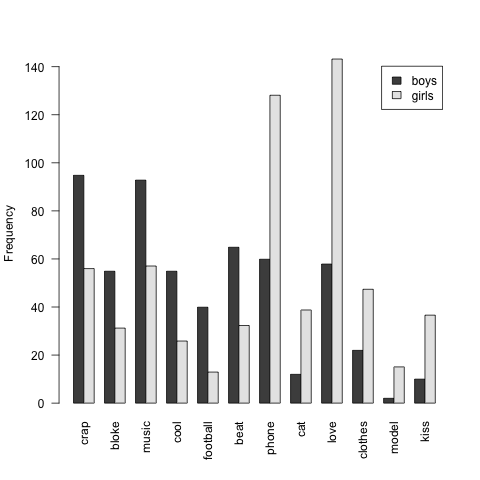
\includegraphics[width=0.7\textwidth]{pics/boysgirls.png}
\caption{Caption of a bar plot} \label{fig:bp}
\end{center} \end{figure}

\section{Regresión}
\label{sec:reg}
Aquí va todos los experimentos de regresión  

\subsection{Red Neuronal de base}
\label{sec:regRedBase}
Aquí va la descripción de la red neuronal de base

\subsection{Búsqueda de hiper-parámetros}
\label{sec:regHiper}
Aquí va la descripción de la búsqueda de hiper-parámetros

\subsection{Red Neuronal Optimizada}
\label{sec:regRedOpt}
Aquí va la descripción de la red neuronal con mejor rendimiento

\subsection{Análisis de las redes neuronales}
\label{sec:regAn}
Aquí va la descripción del análisis de la red neuronal con mejor rendimiento.

Las referencias a figuras se ven así \ref{fig:bpr}. Las figuras están todas en la carpeta pics

\begin{figure}[htbp] \begin{center}
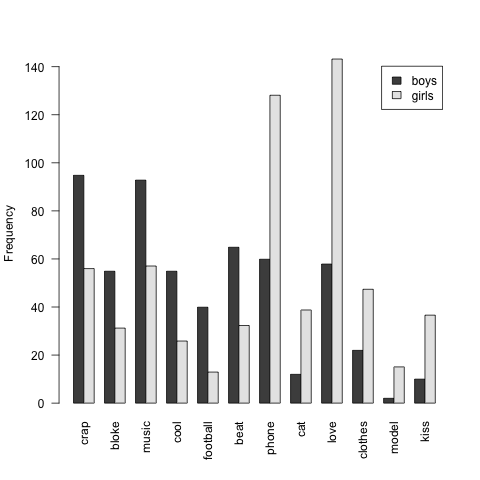
\includegraphics[width=0.7\textwidth]{pics/boysgirls.png}
\caption{Caption of a bar plot} \label{fig:bpr}
\end{center} \end{figure}

\section{Conclusiones}
\label{sec:con}


\printbibliography

\clearpage
\appendix
\section{Apéndice} \label{app:freq}
Aquí va un apéndice

\end{document}